\begin{frame}
	\frametitle{Example of code re-use attack}

	\begin{itemize}
		\item Challenge on ROP Emporium (https://ropemporium.com/)
		\item One executable, split, and a file called "flag.txt"
		\item Make split execute system("/bin/cat flag.txt")
			\begin{itemize}
				\item x86-64
				\item Linux
			\end{itemize}
	\end{itemize}

	\vspace{0.5cm}

	\begin{itemize}
		\item	Buffer Overflow vulnerability
		\item All puzzle pieces are present
		\item	Find an instruction sequence that allows us to set up the arguments
		\item	Overwrite the return address on the stack to hijack control flow
	\end{itemize}

\end{frame}

% Frame with picture
\begin{frame}
	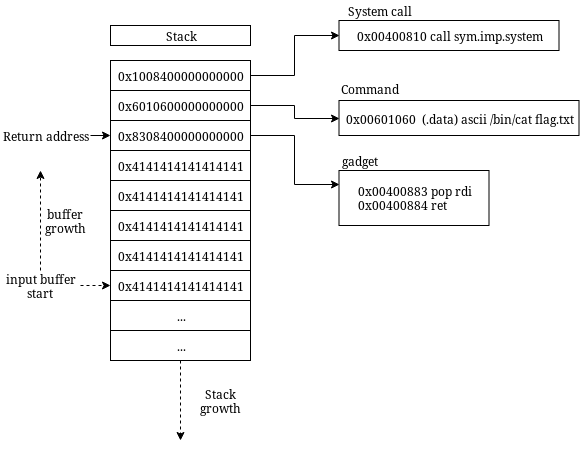
\includegraphics[width=\textwidth]{../background/software-diversity/figures/after-payload}
\end{frame}
